\documentclass[12pt,a4paper]{article}

\usepackage[T1]{fontenc}
\usepackage[utf8]{inputenc}
\usepackage[brazil]{babel}
\usepackage{graphicx}
\usepackage{geometry}
\usepackage{listings}
\usepackage{listingsutf8}
\usepackage{xcolor}
\usepackage{setspace}
\usepackage{float}
\usepackage{tikz}
\usepackage{tabularx}

\usetikzlibrary{positioning, shapes.geometric}
\onehalfspacing
\geometry{margin=2.5cm}

\lstset{
    language=SQL,
    basicstyle=\ttfamily\small,
    keywordstyle=\color{blue},
    commentstyle=\color{gray},
    stringstyle=\color{red},
    breaklines=true,
    showstringspaces=false
}

\newcommand{\montarinicio}[3]{
    % =========================
    % CAPA
    % =========================
    \begin{titlepage}
        \centering

        {\large Faculdade Anhanguera}\\[0.5cm]
        {\large Tecnólogo em DevOps}\\[3cm]

        {\Large \textbf{#1}}\\[2cm]

        {\large Gabriel Blank Stift Mousquer}\\[1cm]

        {\large Ivoti/RS}\\
        {\large 2026}

    \end{titlepage}

    % =========================
    % FOLHA DE ROSTO
    % =========================
    \begin{titlepage}
        \centering

        {\large Faculdade Anhanguera}\\[0.5cm]
        {\large Tecnólogo em DevOps}\\[2cm]

        {\Large \textbf{#1}}\\[1.5cm]

        \begin{flushright}
            Trabalho apresentado à disciplina de \\
            \textbf{#2} \\
            Professor: #3 \\
        \end{flushright}

        \vfill

        {\large Gabriel Blank Stift Mousquer}\\
        Matrícula: 2024201126\\

        \vfill

        {\large Ivoti/RS}\\
        {\large 2026}

    \end{titlepage}

    % =========================
    % SEÇÃO: TOC
    % =========================
    \tableofcontents
    \newpage
}


\begin{document}

\montarinicio
    {OPERADORES E EXPRESSÕES}
    {Algoritmos e Programação Estruturada}
    {Anderson Emídio De Macedo Gonçalves}

\section{Codificação completa}

O código-fonte desenvolvido em linguagem C é apresentado a seguir. Ele implementa a leitura de três números inteiros, a execução das operações aritméticas solicitadas e a verificação das condições utilizando operadores relacionais e lógicos.

\lstset{language=C}

\lstinputlisting[
    caption={Código em C},
    inputencoding=utf8/latin1,
    basicstyle=\ttfamily\scriptsize
]{./static/main.c}

\newpage

\section{Explicação do algoritmo}

O programa desenvolvido solicita três números inteiros ao usuário e aplica operadores aritméticos, relacionais e lógicos conforme proposto.

Foram utilizadas as operações aritméticas básicas: soma (+), subtração (-), multiplicação (*) e divisão (/). A divisão foi realizada com conversão para \texttt{float} para evitar truncamento de resultado. Observa-se que a operação de divisão pode gerar erro em tempo de execução caso o segundo ou o terceiro operando seja igual a zero, situação que não foi tratada por não ser exigida no enunciado.

Os operadores relacionais foram utilizados para verificar se o primeiro número é maior que o segundo (\texttt{>}) e se o segundo número é menor que o terceiro (\texttt{<}), com exibição dos resultados em formato textual.

O operador lógico AND (\texttt{\&\&}) foi aplicado para avaliar simultaneamente duas condições: se o primeiro número é positivo (\texttt{n1 > 0}) e se o segundo número é par (\texttt{n2 \% 2 == 0}). O resultado da expressão lógica também é apresentado ao usuário.

O programa atende aos requisitos propostos, demonstrando o uso direto dos operadores solicitados.

\newpage

\section{Execução do código}

Foram realizados testes com diferentes conjuntos de valores para validar o funcionamento do programa.

\subsection{Caso 1: Entrada (5, 6, 7)}

\begin{figure}[H]
    \centering
    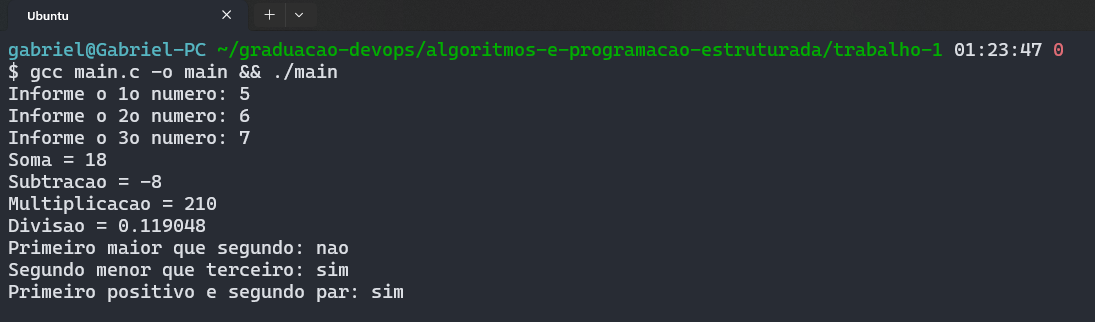
\includegraphics[width=0.8\textwidth]{./static/img-1.png}
\end{figure}

Resultados observados:
\begin{itemize}
    \item Soma: 18, subtração: -8, multiplicação: 210 e divisão com valor decimal.
    \item A condição \texttt{n1 > n2} é falsa.
    \item A condição \texttt{n2 < n3} é verdadeira.
    \item A expressão lógica \texttt{(n1 > 0 \&\& n2 \% 2 == 0)} é verdadeira, pois 5 é positivo e 6 é par.
\end{itemize}

\subsection{Caso 2: Entrada (7, 6, 5)}

\begin{figure}[H]
    \centering
    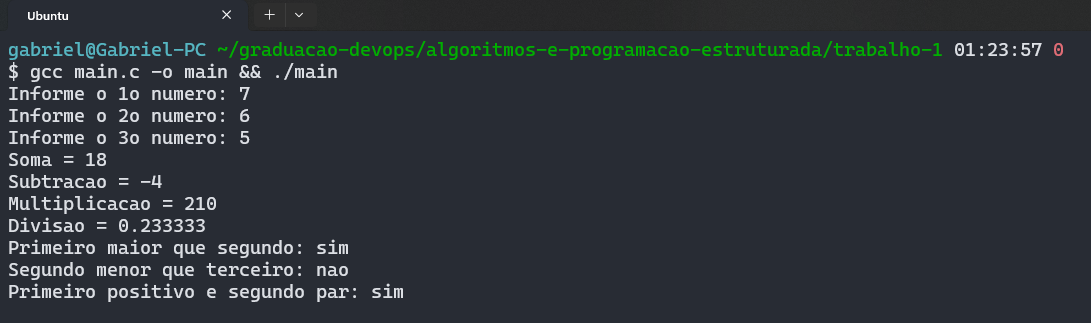
\includegraphics[width=0.8\textwidth]{./static/img-2.png}
\end{figure}

Resultados observados:
\begin{itemize}
    \item Soma: 18, subtração: -4, multiplicação: 210 e divisão com valor decimal.
    \item A condição \texttt{n1 > n2} é verdadeira.
    \item A condição \texttt{n2 < n3} é falsa.
    \item A expressão lógica é verdadeira, pois 7 é positivo e 6 é par.
\end{itemize}

\subsection{Caso 3: Entrada (-10, 2, 2)}

\begin{figure}[H]
    \centering
    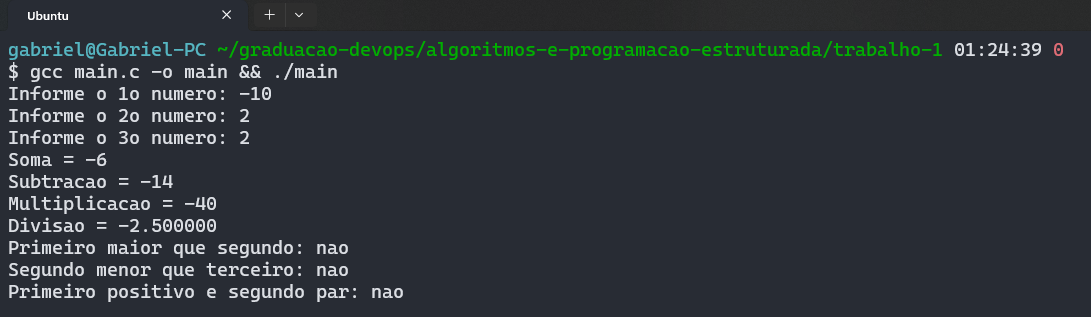
\includegraphics[width=0.8\textwidth]{./static/img-3.png}
\end{figure}

Resultados observados:
\begin{itemize}
    \item Soma: -6, subtração: -14, multiplicação: -40 e divisão com valor decimal.
    \item A condição \texttt{n1 > n2} é falsa.
    \item A condição \texttt{n2 < n3} é falsa.
    \item A expressão lógica é falsa, pois o primeiro número não é positivo.
\end{itemize}

\end{document}
